% lualatex presentation

\documentclass[svgnames]{beamer}
\usepackage{fontspec}
\usepackage{arev}
\usepackage{beramono}
\usepackage{fontawesome}
\usepackage{manfnt}
\usepackage{amsmath}
\usepackage{xcolor}
\usepackage{listings}
\usepackage{hyperref}

\usetheme{default}
\setbeamertemplate{navigation symbols}
{%
%  \hspace{3em}
%  \vbox{%
%  \hbox{\insertslidenavigationsymbol}
%  \hbox{\insertframenavigationsymbol}
%  \hbox{\insertbackfindforwardnavigationsymbol}
%  \vspace{2em}}
}

\setbeamercolor{alerted text}{fg=red!70!black}
\setbeamercolor{structure}{fg=Navy}
\definecolor{wrong}{rgb}{0.7, 0, 0}
\definecolor{right}{rgb}{0, 0.5, 0}
\definecolor{gitred}{rgb}{0.6, 0, 0}
\definecolor{gitgreen}{rgb}{0, 0.5, 0}
\definecolor{gitblue}{rgb}{0, 0, 0.6}
\definecolor{gitbrown}{rgb}{0.6, 0.3, 0}


\hypersetup{%
  pdftitle={Introduction to Version Control with Git}
  ,pdfauthor={Gert-Ludwig Ingold <gert.ingold@physik.uni-augsburg.de>}
  ,pdfsubject={Tutorial at EuroSciPy 2017, Erlangen 29.8.2017}
  ,pdfkeywords={Git, version control system, tutorial, EuroSciPy}
}

\lstset{%
  language={}
  ,basicstyle={\ttfamily\scriptsize}
  ,alsoletter=$
  ,backgroundcolor=\color{black!5}
  ,postbreak=\mbox{\textcolor{gitgreen}{$\hookrightarrow$}\space}
}

\graphicspath{{./images/}}

\begin{document}

\begin{frame}

 \vspace{1truecm}
 \begin{center}
  \structure{\large\textbf{Introduction to Version Control with Git}}\\[0.3truecm]
  \structure{Gert-Ludwig Ingold}

  \vspace{1.5truecm}
  \faicon{github}\ \ttfamily{\scriptsize https://github.com/gertingold/euroscipy-git-tutorial.git}
 \end{center}
\end{frame}

\begin{frame}
 \begin{center}
  \uncover<1->{\bfseries Do you write 100\% bugfree code with all features implemented from the very
	       beginning?\\[0.1truecm]
	       \normalfont yes: 0 points / no: 1 point}

  \vspace{0.2truecm}
  \uncover<2->{\textbullet}

  \vspace{0.2truecm}
  \uncover<2->{\bfseries Do you collaborate with others?\\[0.1truecm]
	       \normalfont yes: 1 point / no: 0 points}

  \vspace{0.2truecm}
  \uncover<3->{\textbullet}

  \vspace{0.2truecm}
  \uncover<3->{\bfseries Do you want to contribute to open software?\\[0.1truecm]
	       \normalfont yes: 1 point / no: 0 points}

  \vspace{0.8truecm}
  \uncover<4>{\alert{\bfseries One or more points: Version control is for you!}}
 \end{center}
\end{frame}

\begin{frame}[fragile]
 \begin{lstlisting}
myscript.py
myscript.py.bak
myscript.py.bak.bak
myscript.py.bak.bak.bak
myscript.py.bak2
myscript.py.bak3
myscript.py.bak4
myscript.py.old
myscript.py.superold
myscript.py.workedonce
paper.tex
paper-20170801.tex
paper-20170725-ab-20170727.tex
paper-20170720-ab-20170721-xy-20170722-ab.tex
paper.tex.old
paper.tex.veryold
paper.tex.firsttry
 \end{lstlisting}

 \uncover<2->{\structure{A big mess. So sad.}}
 
 \vspace{0.2truecm}
 \uncover<3>{\structure{We will use a great VCS. And we will not pay for it.\\ It will be fantastic.}}
\end{frame}

\begin{frame}{A short history of version control}
 \begin{itemize}
  \item \textit{SCCS -- Source Code Control System (1972)}
  \item \textit{RCS -- Revision Control System (1982)}\\
	single file oriented, locking mechanism
  \item \textit{CVS -- Concurrent Versions System (1990)}\\
	\textit{Subversion (2000)}\\
	centralized version control system
  \item \textit{\alert<2>{Git}, Mercurial, Bazaar (2005)}\\
	distributed version control systems
 \end{itemize}

 \begin{center}
  \uncover<2>{
\includegraphics[width=\textwidth]{git_def}}
 \end{center}
\end{frame}

\begin{frame}{Centralized version control systems}
 \begin{center}
  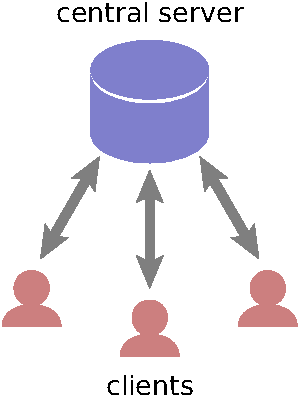
\includegraphics[width=\textwidth]{cvcs}
 \end{center}

 At any time, the central server contains well defined revisions
 of file sets which can be consecutively numbered.
\end{frame}

\begin{frame}{Distributed version control systems}
 \begin{center}
  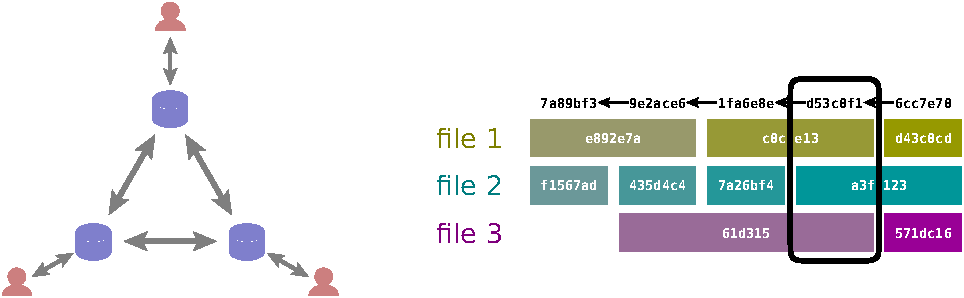
\includegraphics[width=\textwidth]{dvcs}
 \end{center}

 \begin{itemize}
  \item each individual repository has its own history
  \item each object is identified by a SHA1 hash consisting of
	40 hexadecimal values
  \item there are more than $10^{48}$ different SHA1 hashes
  \item often the first seven hex digits are sufficient for identification
 \end{itemize}
\end{frame}

\begin{frame}{Distributed VCS with Gitlab / Github}
 \begin{center}
  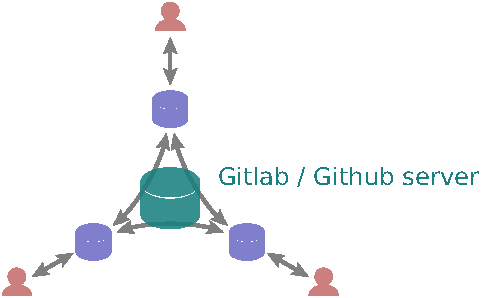
\includegraphics[height=0.6\textheight]{dvcs-github}
 \end{center}
\end{frame}

\begin{frame}{Where to get the software and more information}
 \begin{columns}
  \begin{column}{0.5\textwidth}
   \structure{\large\texttt{https://git-scm.com/}}

   \vspace{2truecm}
  \end{column}%
  \begin{column}{0.5\textwidth}
   \begin{center}
    
\includegraphics[width=\textwidth]{gitscm}
   \end{center}
  \end{column}%
 \end{columns}

 \begin{itemize}
  \item binaries for Windows and Mac OS X, install instructions for
        Linux and Solaris
  \item reference documentation
  \item online version of the \textit{Pro Git} book by S. Chacon and B.  Straub
        including several translations
  \item some instructional videos
  \item and more \dots
 \end{itemize}
\end{frame}

\begin{frame}[fragile]{How to get help: \texttt{git help}}
 \begin{lstlisting}[basicstyle={\ttfamily\tiny}]
$ git help
These are common Git commands used in various situations:

start a working area (see also: git help tutorial)
   clone      Clone a repository into a new directory
   init       Create an empty Git repository or reinitialize an existing one

work on the current change (see also: git help everyday)
   add        Add file contents to the index
   mv         Move or rename a file, a directory, or a symlink
   reset      Reset current HEAD to the specified state
   rm         Remove files from the working tree and from the index

examine the history and state (see also: git help revisions)
   bisect     Use binary search to find the commit that introduced a bug
   grep       Print lines matching a pattern
   log        Show commit logs
   show       Show various types of objects
   status     Show the working tree status

grow, mark and tweak your common history
   branch     List, create, or delete branches
   checkout   Switch branches or restore working tree files
   commit     Record changes to the repository
   diff       Show changes between commits, commit and working tree, etc
   merge      Join two or more development histories together
   rebase     Reapply commits on top of another base tip
   tag        Create, list, delete or verify a tag object signed with GPG

collaborate (see also: git help workflows)
   fetch      Download objects and refs from another repository
   pull       Fetch from and integrate with another repository or a local branch
   push       Update remote refs along with associated objects
 \end{lstlisting}
\end{frame}

\begin{frame}[fragile]{How to get help on a specific command}

 \structure{\texttt{git help <command>}}
 \addtolength\linewidth{0.5truecm}
 \begin{lstlisting}[basicstyle={\ttfamily\tiny}]
$ git help add
NAME
       git-add - Add file contents to the index

SYNOPSIS
       git add [--verbose | -v] [--dry-run | -n] [--force | -f] [--interactive | -i]
                 [--patch | -p] [--edit | -e] [--[no-]all | --[no-]ignore-removal |
                 [--update | -u]] [--intent-to-add | -N] [--refresh] [--ignore-errors]
                 [--ignore-missing] [--chmod=(+|-)x] [--] [<pathspec>...]

DESCRIPTION

       This command updates the index using the current content found in the working
       tree, to prepare the content staged for the next commit. It typically adds
       the current content of existing paths as a whole, but with some options it
       can also be used to add content with only part of the changes made to the
       working tree files applied, or remove paths that do not exist in the working
       tree anymore.

...
 \end{lstlisting}
\end{frame}

\begin{frame}[fragile]{Accessing Git tutorials}
 \begin{lstlisting}[basicstyle={\ttfamily\tiny}]
$ git help -g
The common Git guides are:

   attributes   Defining attributes per path
   everyday     Everyday Git With 20 Commands Or So
   glossary     A Git glossary
   ignore       Specifies intentionally untracked files to ignore
   modules      Defining submodule properties
   revisions    Specifying revisions and ranges for Git
   tutorial     A tutorial introduction to Git (for version 1.5.1 or newer)
   workflows    An overview of recommended workflows with Git

'git help -a' and 'git help -g' list available subcommands and some
concept guides. See 'git help <command>' or 'git help <concept>'
to read about a specific subcommand or concept.
 \end{lstlisting}
 \begin{lstlisting}[basicstyle={\ttfamily\tiny}, escapechar=\%]
$git help everyday

NAME
       giteveryday - A useful minimum set of commands for Everyday Git

SYNOPSIS
       Everyday Git With 20 Commands Or So

DESCRIPTION
       Git users can broadly be grouped into four categories for the purposes of
       describing here a small set of useful command for everyday Git.

       %\cdot%   Individual Developer (Standalone) commands are essential for anybody who
           makes a commit, even for somebody who works alone.

       %\cdot%   If you work with other people, you will need commands listed in the
           Individual Developer (Participant) section as well.
...
 \end{lstlisting}
\end{frame}

\begin{frame}{The prime time project}
 \textit{\structure{Question}}

 How many prime numbers can be interpreted as time in the format HH:MM?

 \vspace{1\baselineskip}
 \textit{\structure{Examples}}

 \textcolor{wrong}{2179 is a prime, but 21:79 is not a valid time}\\
 \textcolor{right}{2137 is a prime and 21:37 is a valid time}\\
 \textcolor{right}{953 is a prime and 9:53 is a valid time}\\
 \textcolor{wrong}{89 is a prime, but 0:89 is not a valid time}\\
 \textcolor{right}{41 is a prime and 0:41 is a valid time}\\
 \textcolor{right}{7 is a prime and 0:07 is a valid time}

 \vspace{1.5\baselineskip}
 \begin{center}
 \uncover<2>{\structure{\bfseries And, of course, we are going to use\\ a Git repository.}}
 \end{center}
\end{frame}

\begin{frame}[fragile]{Creating a respository}
 \structure{Initializing a new repository}

 \begin{lstlisting}
~/primetime$ git init
 \end{lstlisting}

 \vspace{\baselineskip}
 \structure{What has happened?}
 \begin{lstlisting}
~/primetime$ ls -a
.  ..  .git
~/primetime$ ls .git
branches  description  hooks  objects
config    HEAD         info   refs
 \end{lstlisting}

 \begin{center}
  \uncover<2>{\alert{\raisebox{0.5em}{\dbend}\quad Keep your hands off the \texttt{.git} directory!!!}}
 \end{center}
\end{frame}

\begin{frame}[fragile]{Tell Git who you are}

 \structure{Specify your name and your email address}
 \begin{lstlisting}
$ git config --global user.name <your name>
$ git config --global user.email <your email>
 \end{lstlisting}

 \vspace{\baselineskip}
 \structure{\ldots and, if you want, your preferred editor}
 \begin{lstlisting}
$ git config --global core.editor <editor>
 \end{lstlisting}

 \vspace{\baselineskip}
 \structure{example configuration}
 \begin{lstlisting}
$ git config --list
user.email=gert.ingold@physik.uni-augsburg.de
user.name=Gert-Ludwig Ingold
core.editor=vim
...
 \end{lstlisting}
\end{frame}

\begin{frame}[fragile]{It's prime time now}
 \texttt{primetime.py}
 \begin{lstlisting}
def istime(n):
    hh, mm = divmod(n, 100)
    return 0 <= hh <= 23 and 0 <= mm <= 59

print(sum(istime(n) for n in range(2360)))
 \end{lstlisting}

 \vspace{0.2truecm}
 \structure{What is the status?}
 \begin{lstlisting}[breaklines=true
                    ,escapechar=\%]
~/primetime$ git status
On branch master

Initial commit

Untracked files:
  (use "git add <file>..." to include in what will be committed)

        %\textcolor{gitred}{primetime.py}%

nothing added to commit but untracked files present (use "git add" to track)
 \end{lstlisting}
 \begin{itemize}
  \item Git has noticed our new file but ignores it
  \item Git tells us how to put the file under version control
 \end{itemize}
\end{frame}

\begin{frame}[fragile]{Adding a file}
 \begin{lstlisting}
~/primetime$ git add primetime.py
 \end{lstlisting}

 \vspace{0.2truecm}
 \structure{How did the status change?}
 \begin{lstlisting}[escapechar=\%]
~/primetime$ git status
On branch master

Initial commit

Changes to be committed:
  (use "git rm --cached <file>..." to unstage)

        %\textcolor{gitgreen}{new file:}%   %\textcolor{gitgreen}{primetime.py}%
 \end{lstlisting}
 \begin{itemize}
  \item Our file is now in the staging area, \alert{it is not under version control yet!}
  \item Our file can now be committed, but we can add more files first
  \item Git tells us how we can remove the file from the staging area if we put
        it there by accident
 \end{itemize}
\end{frame}

\begin{frame}{The way into the repository}
 \begin{center}
  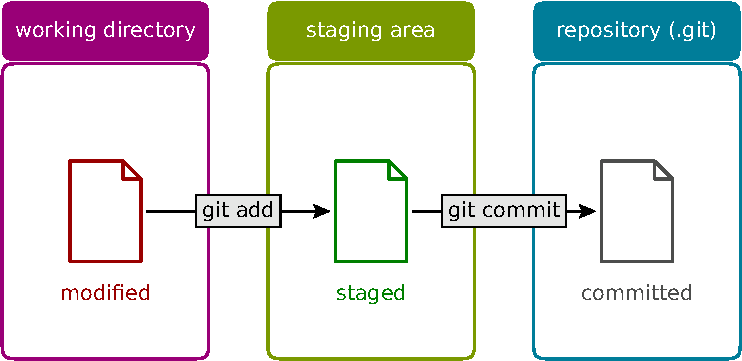
\includegraphics[width=0.9\textwidth]{addcommit}
 \end{center}
 \begin{itemize}
  \item All files present in the staging area are committed
  \item At a given time, different versions of a specific file can exist in
	any of the three areas
 \end{itemize}
\end{frame}

\begin{frame}[fragile]{Committing a file}
 \begin{lstlisting}
~/primetime$ git commit -m'added function to identify times'
[master (root-commit) 3733ef5] added function to identify times
 1 file changed, 5 insertions(+)
 create mode 100644 primetime.py
 \end{lstlisting}
 \begin{itemize}
  \item The option \texttt{-m} allows to specify a commit message
  \item Without this option, an editor is opened
  \item Limit the commit message to 50 characters
 \end{itemize}

 \vspace{0.2truecm}
 \structure{Check status to make sure that everything is fine}
 \begin{lstlisting}
~/primetime$ git status
On branch master
nothing to commit, working tree clean
 \end{lstlisting}
\end{frame}

\begin{frame}{Some tips on committing}
 \begin{itemize}
  \item A commit can contain several files, but all changes should
	represent a logical unit
  \item \textit{atomic commit:} Each commit refers only to a single
	basic change
  \item In most cases it is not a good idea to commit only at the
	end of a long working day
  \item If you have made unrelated changes but want to do an atomic
	commit, take a look at\\ \texttt{git add -p}
 \end{itemize}
\end{frame}

\begin{frame}[fragile]{A first complete version of primetime}
 \texttt{primes.py} (very inefficient)
 \begin{lstlisting}
def isprime(n):
    if n < 2: return False
    for divisor in range(2, n):
        if not n % divisor:
            return False
    return True
 \end{lstlisting}

 \vspace{0.2truecm}
 \texttt{primetime.py}
 \begin{lstlisting}
from primes import isprime

def istime(n):
    hh, mm = divmod(n, 100)
    return 0 <= hh <= 23 and 0 <= mm <= 59

print(sum(isprime(n) for n in range(2360) if istime(n)))
 \end{lstlisting}

 \vspace{0.4truecm}
 \structure{It works:}
 \begin{lstlisting}
~/primetime$ python primetime.py
211 
 \end{lstlisting}
\end{frame}

\begin{frame}[fragile]{The new status}
 \addtolength\linewidth{0.5truecm}
 \begin{lstlisting}[breaklines=true, escapechar=\%]
~/primetime$ git status
On branch master
Changes not staged for commit:
  (use "git add <file>..." to update what will be committed)
  (use "git checkout -- <file>..." to discard changes in working directory)

        modified:   %\textcolor{gitred}{primetime.py}%

Untracked files:
  (use "git add <file>..." to include in what will be committed)

        %\textcolor{gitred}{\_\_pycache\_\_/}%
        %\textcolor{gitred}{primes.py}%

no changes added to commit (use "git add" and/or "git commit -a")
 \end{lstlisting}
 \begin{itemize}
  \item Git noticed that \texttt{primetime.py} has been modified
  \item \texttt{primes.py} is new and not yet tracked by Git
  \item The directory \texttt{\_\_pycache\_\_/} should not be under version control
  \item Note also the help given by Git
 \end{itemize}
\end{frame}

\begin{frame}[fragile]{The \texttt{.gitignore} file}
 \begin{itemize}
  \item List in \texttt{.gitignore} line-by-line all directories and files to
	be ignored by Git
  \item * can be used as a wildcard
  \item Everything after a \# is a comment
  \item Put \texttt{.gitignore} under version control
  \item \texttt{.gitignore} can help to make sure that passwords never are put
	under version control
 \end{itemize}

 \vspace{0.3truecm}
 In our example:\\
 \texttt{.gitignore}
 \begin{lstlisting}
__pycache__/
 \end{lstlisting}
\end{frame}

\begin{frame}[fragile]{Add and commit}
 \begin{lstlisting}
~/primetime$ git add .gitignore
~/primetime$ git commit -m'.gitignore added'
[master c552c10] .gitignore added
 1 file changed, 1 insertion(+)
 create mode 100644 .gitignore
 \end{lstlisting}
 \begin{lstlisting}[escapechar=\%]
~/primetime$ git add primetime.py
~/primetime$ git add primes.py
~/primetime$ git status
On branch master
Changes to be committed:
  (use "git reset HEAD <file>..." to unstage)

        new file:   %\textcolor{gitgreen}{primes.py}%
        modified:   %\textcolor{gitgreen}{primetime.py}%

~/primetime$ git commit -m'first version of primetime completed'
[master 116fd26] first version of primetime completed
 2 files changed, 9 insertions(+), 1 deletion(-)
 create mode 100644 primes.py
 \end{lstlisting}
\end{frame}

\begin{frame}[fragile]{Branches}
 \begin{lstlisting}
~/primetime$ git status
On branch master
nothing to commit, working tree clean
 \end{lstlisting}
 \begin{itemize}
  \item We are on branch \texttt{master}, the default branch
 \end{itemize}
 \begin{lstlisting}[escapechar=\%]
gert@gli7440:~/primetime$ git branch
* %\textcolor{gitgreen}{master}%
 \end{lstlisting}
 \structure{What are branches good for?}
 \begin{itemize}
  \item Branches allow development of features without polluting
        the master branch
  \item Tip: Use a separate branch for each feature
  \item Unsuccessful experiments can easily be removed by deleting
        a branch
  \item In collaborative work, a pull request (see later) can easily
        focus on the new code
  \item Code can be merged into other branches
 \end{itemize}
\end{frame}

\begin{frame}[fragile]{Adding a new branch}
 In our prime time project, we are unhappy with our code for prime tests.
 Instead, we want to create a list of primes by means of the sieve of
 Eratosthenes. We develop the new feature in a separate branch so that the
 version in the master branch is always working.

 \begin{lstlisting}[breaklines=true]
~/primetime$ git checkout eratosthenes
error: pathspec 'eratosthenes' did not match any file(s) known to git.
 \end{lstlisting}
 \begin{itemize}
  \item \texttt{git checkout} changes between branches, but our branch
        does not yet exist. Use option \texttt{-b}
 \end{itemize}
 \begin{lstlisting}
gert@gli7440:~/primetime$ git checkout -b eratosthenes
Switched to a new branch 'eratosthenes'
 \end{lstlisting}

 \vspace{0.2truecm}
 Let us verify the branch
 \begin{lstlisting}[escapechar=\%]
gert@gli7440:~/primetime$ git branch
* %\textcolor{gitgreen}{eratosthenes}%
  master
 \end{lstlisting}
\end{frame}

\begin{frame}[fragile]{Improved primetime code (I)}
 \texttt{primes.py}
 \begin{lstlisting}
from math import sqrt
import numpy as np

def isprime(n):
    if n < 2: return False
    for divisor in range(2, n):
        if not n % divisor:
            return False
    return True

def eratosthenes(nmax):
    sieve = np.ones(nmax+1, dtype=np.bool)
    sieve[:2] = False
    for candidate in range(2, int(sqrt(nmax))+1):
        if sieve[candidate]:
            sieve[candidate*candidate::candidate] = False
    primes = np.arange(nmax+1)[sieve]
    return primes
 \end{lstlisting}
 \begin{lstlisting}
~/primetime$ git commit -a -m'added sieve of Eratosthenes'
[eratosthenes 982ae11] added sieve of Eratosthenes
 1 file changed, 12 insertions(+)
 \end{lstlisting}
\end{frame}

\begin{frame}[fragile]{Improved primetime code (II)}
 \addtolength\linewidth{0.7truecm}
 \texttt{primetime.py}
 \begin{lstlisting}
from primes import eratosthenes

def istime(n):
    hh, mm = divmod(n, 100)
    return 0 <= hh <= 23 and 0 <= mm <= 59

print(sum(istime(n) for n in eratosthenes(2359)))
 \end{lstlisting}
 \begin{lstlisting}
~/primetime$ git commit -a -m'make use of Eratosthenes in primetime'
[eratosthenes c9dfe03] make use of Eratosthenes in primetime
 1 file changed, 2 insertions(+), 2 deletions(-)
 \end{lstlisting}
\end{frame}

\begin{frame}[fragile]{Working on branches in parallel}
 In the meantime, an idea comes up to improve the function \texttt{isprime}.
 We make the corresponding changes in the master branch.

 First switch to the master branch:
 \begin{lstlisting}
~/primetime$ git checkout master
Switched to branch 'master'
 \end{lstlisting}

 Here, \texttt{primes.py} does not contain the function \texttt{eratosthenes}.
 We replace the code by
 \begin{lstlisting}
from math import sqrt

def isprime(n):
    if n < 2: return False
    for divisor in range(2, int(sqrt(n))+1):
        if not n % divisor:
            return False
    return True
 \end{lstlisting}
 \begin{lstlisting}
~/primetime$ git commit -a -m'improved prime test'
[master ebc424d] improved prime test
 1 file changed, 3 insertions(+), 1 deletion(-)
 \end{lstlisting}
\end{frame}

\begin{frame}[fragile]{Commits in different branches}
 \addtolength\linewidth{0.5truecm}
 \begin{lstlisting}[escapechar=\%]
~/primetime$ git log  --graph --branches --oneline
* %\textcolor{gitbrown}{ebc424d}% improved prime test
%\textcolor{gitred}{|}% * %\textcolor{gitbrown}{c9dfe03}% make use of Eratosthenes in primetime
%\textcolor{gitred}{|}% * %\textcolor{gitbrown}{982ae11}% added sieve of Eratosthenes
%\textcolor{gitred}{|/}%  
* %\textcolor{gitbrown}{116fd26}% first version of primetime completed
* %\textcolor{gitbrown}{c552c10}% .gitignore added
* %\textcolor{gitbrown}{3733ef5}% added function to identify times
 \end{lstlisting}

 \vspace{0.2truecm}
 \structure{Merging the content of the \texttt{eratosthenes} branch into the \texttt{master}
            branch}
 \begin{lstlisting}[escapechar=\%]
~/primetime$ git branch
  eratosthenes
  * %\textcolor{gitgreen}{master}%
  ~/primetime$ git merge eratosthenes
  Auto-merging primes.py
  CONFLICT (content): Merge conflict in primes.py
  Automatic merge failed; fix conflicts and then commit the result.
 \end{lstlisting}
 \begin{itemize}
  \item \texttt{primetime.py} corresponds now to the \texttt{eratosthenes} branch
  \item In \texttt{primes.py} a merge conflict needs to be resolved
 \end{itemize}
\end{frame}

\begin{frame}[fragile]{A merge conflict}
 \begin{lstlisting}[escapeinside=`´]
from math import sqrt
`\textcolor{red}{<\/<\/<\/<\/<\/<\/< HEAD}´
`\textcolor{red}{=======}´
`\textcolor{red}{import numpy as np}´
`\textcolor{red}{>\/>\/>\/>\/>\/>\/> eratosthenes}´

def isprime(n):
    if n < 2: return False
    for divisor in range(2, int(sqrt(n))+1):
        if not n % divisor:
            return False
    return True

def eratosthenes(nmax):
...
 \end{lstlisting}
 \begin{itemize}
  \item Alternative 1 between \texttt{>\/>\/>\/>\/>\/>\/>} and \texttt{=======}\\
	\texttt{HEAD} = version being merged into

  \item Alternative 2 between \texttt{=======} and \texttt{<\/<\/<\/<\/<\/<\/<}\\
	\texttt{eratosthenes} = version being merged
  \item Bring the file into the desired form and commit it
 \end{itemize}
\end{frame}

\begin{frame}[fragile]{Resolving a merge conflict}
 new version of \texttt{primes.py}
 \begin{lstlisting}
from math import sqrt
import numpy as np

def isprime(n):
    if n < 2: return False
...
 \end{lstlisting}
 \begin{lstlisting}
~/primetime$ git commit -a
[master 5782233] Merge branch 'eratosthenes'
 \end{lstlisting}
 \begin{lstlisting}[escapechar=\%]
~/primetime$ git log --graph --branches --oneline
*   %\textcolor{gitbrown}{5782233}% Merge branch 'eratosthenes'
%\textcolor{gitred}{|}\textcolor{gitgreen}{\textbackslash}%  
%\textcolor{gitred}{|}% * %\textcolor{gitbrown}{c9dfe03}% make use of Eratosthenes in primetime
%\textcolor{gitred}{| }%* %\textcolor{gitbrown}{982ae11}% added sieve of Eratosthenes
* %\textcolor{gitgreen}{|}% %\textcolor{gitbrown}{ebc424d}% improved prime test
%\textcolor{gitgreen}{|/}%  
* %\textcolor{gitbrown}{116fd26}% first version of primetime completed
* %\textcolor{gitbrown}{c552c10}% .gitignore added
* %\textcolor{gitbrown}{3733ef5}% added function to identify times
 \end{lstlisting}
\end{frame}

\begin{frame}[fragile]{Deleting a branch}
 \begin{lstlisting}
~/primetime$ git branch -D eratosthenes
Deleted branch eratosthenes (was c9dfe03).
 \end{lstlisting}
 \begin{itemize}
  \item option D must be uppercase = \alert{Attention, danger!}
 \end{itemize}
 \begin{lstlisting}[escapechar=\%]
~/primetime$ git branch
* %\textcolor{gitgreen}{master}%
 \end{lstlisting}
 \begin{itemize}
  \item The old versions still exist
 \end{itemize}
 \begin{lstlisting}[escapechar=\%]
~/primetime$ git log --graph --branches --oneline
*   %\textcolor{gitbrown}{5782233}% Merge branch 'eratosthenes'
%\textcolor{gitred}{|}\textcolor{gitgreen}{\textbackslash}%  
%\textcolor{gitred}{|}% * %\textcolor{gitbrown}{c9dfe03}% make use of Eratosthenes in primetime
%\textcolor{gitred}{| }%* %\textcolor{gitbrown}{982ae11}% added sieve of Eratosthenes
* %\textcolor{gitgreen}{|}% %\textcolor{gitbrown}{ebc424d}% improved prime test
%\textcolor{gitgreen}{|/}%  
* %\textcolor{gitbrown}{116fd26}% first version of primetime completed
* %\textcolor{gitbrown}{c552c10}% .gitignore added
* %\textcolor{gitbrown}{3733ef5}% added function to identify times
 \end{lstlisting}
\end{frame}

\begin{frame}[fragile]{Accessing a specific version}
 \begin{lstlisting}[escapechar=\%]
~/primetime$ git log --oneline --graph --branches --decorate
*   %\textcolor{gitbrown}{5782233 (}\textcolor{gitblue}{HEAD ->} \textcolor{gitgreen}{master}\textcolor{gitbrown}{)}% Merge branch 'eratosthenes'
%\textcolor{gitred}{|}\textcolor{gitgreen}{\textbackslash}%  
%\textcolor{gitred}{|} * \textcolor{gitbrown}{c9dfe03}% make use of Eratosthenes in primetime
%\textcolor{gitred}{|} * \textcolor{gitbrown}{982ae11}% added sieve of Eratosthenes
* %\textcolor{gitgreen}{|} \textcolor{gitbrown}{ebc424d}% improved prime test
%\textcolor{gitgreen}{|/}%  
* %\textcolor{gitbrown}{116fd26}% first version of primetime completed
* %\textcolor{gitbrown}{c552c10}% .gitignore added
* %\textcolor{gitbrown}{3733ef5}% added function to identify times
 \end{lstlisting}
 \begin{itemize}
  \item absolute reference: HEAD or SHA1 hash
  \item relative reference:\\[0.1truecm]
        \begin{tabular}{lll}
         parent & HEAD\textasciicircum & \texttt{ebc424d}\\
         parent & c552c10\textasciicircum & \texttt{3733ef5}\\
         2nd parent & HEAD\textasciicircum2 & \texttt{c9dfe03}\\
         grandparent & HEAD\textasciicircum\textasciicircum & \texttt{116fd26}\\
         grandparent & HEAD\textasciitilde2 & \texttt{116fd26}\\
        \end{tabular}
 \end{itemize}
\end{frame}

\begin{frame}[fragile]{Detached HEAD}
 \begin{lstlisting}[basicstyle={\ttfamily\tiny}]
~/primetime$ git checkout 982ae11
Note: checking out '982ae11'.

You are in 'detached HEAD' state. You can look around, make experimental
changes and commit them, and you can discard any commits you make in this
state without impacting any branches by performing another checkout.

If you want to create a new branch to retain commits you create, you may
do so (now or later) by using -b with the checkout command again. Example:

  git checkout -b <new-branch-name>

HEAD is now at 982ae11... added sieve of Eratosthenes
 \end{lstlisting}

 \begin{lstlisting}[escapechar=\%]
~/primetime$ git log --oneline --graph --branches --decorate
*   %\textcolor{gitbrown}{5782233 (}\textcolor{gitgreen}{master}\textcolor{gitbrown}{)}% Merge branch 'eratosthenes'
%\textcolor{gitred}{|}\textcolor{gitgreen}{\textbackslash}%  
%\textcolor{gitred}{|} * \textcolor{gitbrown}{c9dfe03}% make use of Eratosthenes in primetime
%\textcolor{gitred}{|} * \textcolor{gitbrown}{982ae11 (}\textcolor{gitblue}{HEAD}\textcolor{gitbrown}{)}% added sieve of Eratosthenes
* %\textcolor{gitgreen}{|} \textcolor{gitbrown}{ebc424d}% improved prime test
%\textcolor{gitgreen}{|/}%  
* %\textcolor{gitbrown}{116fd26}% first version of primetime completed
* %\textcolor{gitbrown}{c552c10}% .gitignore added
* %\textcolor{gitbrown}{3733ef5}% added function to identify times
 \end{lstlisting}

 \begin{itemize}
  \item HEAD is not attached to a branch, it is detached
  \item In order to commit something, a branch needs to be created
 \end{itemize}
\end{frame}

\begin{frame}[fragile]{Attaching HEAD to a branch}
 \begin{lstlisting}[escapechar=\%]
~/primetime$ git branch
* %\textcolor{gitgreen}{(HEAD detached at 982ae11)}%
  master
 \end{lstlisting}
 \begin{lstlisting}[escapechar=\%]
~/primetime$ git checkout -b experimental
Switched to a new branch 'experimental'
~/primetime$ git branch -v
* %\textcolor{gitgreen}{experimental}% 982ae11 added sieve of Eratosthenes
  master       5782233 Merge branch 'eratosthenes'
 \end{lstlisting}
 \begin{itemize}
  \item Now we have a branch at \texttt{982ae11} on which we can work and commit
        changes
 \end{itemize}
\end{frame}

\begin{frame}[fragile]{Tagging versions}
 Sometimes it is useful to mark a specific version, e.g. the submitted version of a paper.

 \vspace{0.2truecm}
 \structure{Tagging the present version}
 \begin{lstlisting}[breaklines=true]
~/primetime$ git tag -a first_final -m'a first reasonably complete version'
 \end{lstlisting}

 \structure{Tagging an older version}
 \begin{lstlisting}
~/primetime$ git tag -a v0.1 116fd26 -m'early version'
 \end{lstlisting}

 \begin{lstlisting}
~/primetime$ git tag
first_final
v0.1
 \end{lstlisting}

 \begin{lstlisting}[basicstyle={\ttfamily\tiny}]
~/primetime$ git show v0.1
tag v0.1
Tagger: Gert-Ludwig Ingold <gert.ingold@physik.uni-augsburg.de>
Date:   Mon Aug 14 01:12:07 2017 +0200

early version

commit 116fd26220dddb7ec3eb359d3c35ea9c312bb49c
Author: Gert-Ludwig Ingold <gert.ingold@physik.uni-augsburg.de>
Date:   Sun Aug 13 16:16:46 2017 +0200

    first version of primetime completed

...
 \end{lstlisting}
\end{frame}

\begin{frame}{Working with Github}
 \begin{center}
  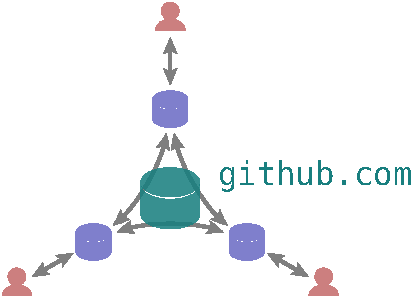
\includegraphics[width=0.5\textwidth]{github}
 \end{center}

 \structure{What is Github?}
 \begin{itemize}
  \item Github hosts Git projects and facilitates collaborative development by means of Git
  \item \textit{Public} repositories readable for everybody are available free of charge
  \item \textit{Private} repositories are not free, but may be free for academic use on request
  \item Github is very popular for open source projects
 \end{itemize}
\end{frame}

\begin{frame}[fragile]{Cloning a repository}
 \structure{Scenario:} You want to get the content of a repository without contributing
	to its development.

 \begin{lstlisting}[basicstyle={\ttfamily\tiny}]
$ git clone https://github.com/gertingold/euroscipy-git-tutorial.git
Cloning into 'euroscipy-git-tutorial'...
remote: Counting objects: 205, done.
remote: Compressing objects: 100% (30/30), done.
remote: Total 205 (delta 40), reused 61 (delta 37), pack-reused 138
Receiving objects: 100% (205/205), 354.93 KiB | 0 bytes/s, done.
Resolving deltas: 100% (121/121), done.
Checking connectivity... done.
 \end{lstlisting}

 \begin{lstlisting}[basicstyle={\ttfamily\tiny}]
$ ls euroscipy-git-tutorial/
images  LICENSE  presentation.tex  README.md
 \end{lstlisting}

 or if you just want the current version
 \begin{lstlisting}[basicstyle={\ttfamily\tiny}
                    ,escapechar=\|
                   ]
$ git clone |\alert{\texttt{-\/-depth=1}}| https://github.com/gertingold/euroscipy-git-tutorial.git
Cloning into 'euroscipy-git-tutorial'...
remote: Counting objects: 23, done.
remote: Compressing objects: 100% (23/23), done.
remote: Total 23 (delta 3), reused 14 (delta 0), pack-reused 0
Unpacking objects: 100% (23/23), done.
Checking connectivity... done.
$ ls euroscipy-git-tutorial/
images  LICENSE  presentation.tex  README.md
 \end{lstlisting}

\end{frame}

\begin{frame}{Typical workflow for project development}
 \structure{Scenario:} You want to contribute to a project, but only the maintainers
	can make changes to the repository.

 \vspace{0.3truecm}
 \only<1>{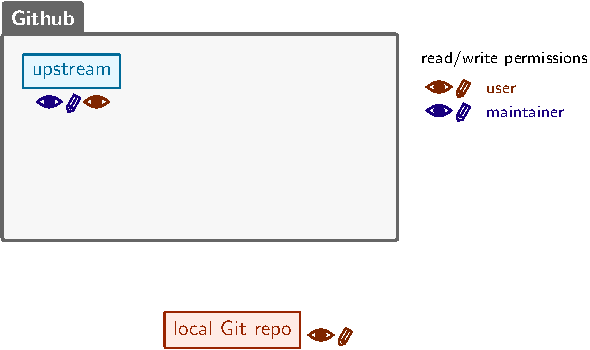
\includegraphics[width=\textwidth]{github-oss_1}}%
 \only<2>{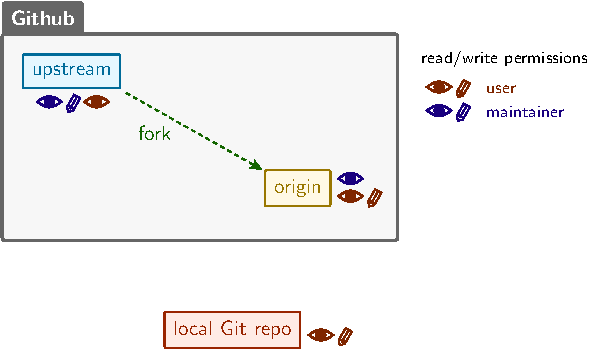
\includegraphics[width=\textwidth]{github-oss_2}}%
 \only<3>{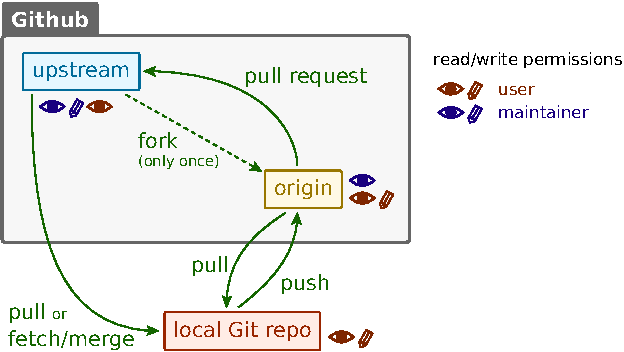
\includegraphics[width=\textwidth]{github-oss_3}}
\end{frame}

\begin{frame}{Remote branches}
\end{frame}

\end{document}
